\documentclass[11pt,a4paper]{ivoa}
\input tthdefs

\title{Catalogue of User Defined Functions}

% see ivoatexDoc for what group names to use here
\ivoagroup{DAL}

%\author[????URL????]{????Alfred Usher Thor????}
\author{Markus Demleitner}
\author{Jon Juaristi Campillo}


\editor{Markus Demleitner}

% \previousversion[????URL????]{????Funny Label????}
\previousversion{This is the first public release}
       

\begin{document}
\begin{abstract}
In these document the official IVOA sanctioned User Defined Functions
(UDF) are listed. The functions must be prefixed by ``ivo\_`` as
defined in the standard. Should more be defined for future use, they
will be written down in this note.
\end{abstract}


%i\section*{Acknowledgments}

%???? Or remove the section header ????

\section*{Conformance-related definitions}

The words ``MUST'', ``SHALL'', ``SHOULD'', ``MAY'', ``RECOMMENDED'', and
``OPTIONAL'' (in upper or lower case) used in this document are to be
interpreted as described in IETF standard RFC2119 \citep{std:RFC2119}.

The \emph{Virtual Observatory (VO)} is a
general term for a collection of federated resources that can be used
to conduct astronomical research, education, and outreach.
The \href{http://www.ivoa.net}{International
Virtual Observatory Alliance (IVOA)} is a global
collaboration of separately funded projects to develop standards and
infrastructure that enable VO applications.


\section{Introduction}

After more than a decade since the foundation of the IVOA, multiple
Virtual Observatories across the world have adapted its standards. In
this case, TAP and its query language, ADQL. Due to some of the
functionality not being present in the standards, IVOA defined some UDF
which help users obtain HealPix maps for instance. Despite this, and due
to different services working in different context, there is disparity
on UDF.

In this note we intend to compile those which can be service-independent
but adoptable by anyone who deems it necessary.

%\subsection{Role within the VO Architecture}

%\begin{figure}
%\centering

%% As of ivoatex 1.2, the architecture diagram is generated by ivoatex in
% SVG; copy ivoatex/archdiag-full.xml to archdiag.xml and throw out
% all lines not relevant to your standard.
% Notes don't generally need this.  If you don't copy archdiag.xml,
% you must remove archdiag.svg from FIGURES in the Makefile.

%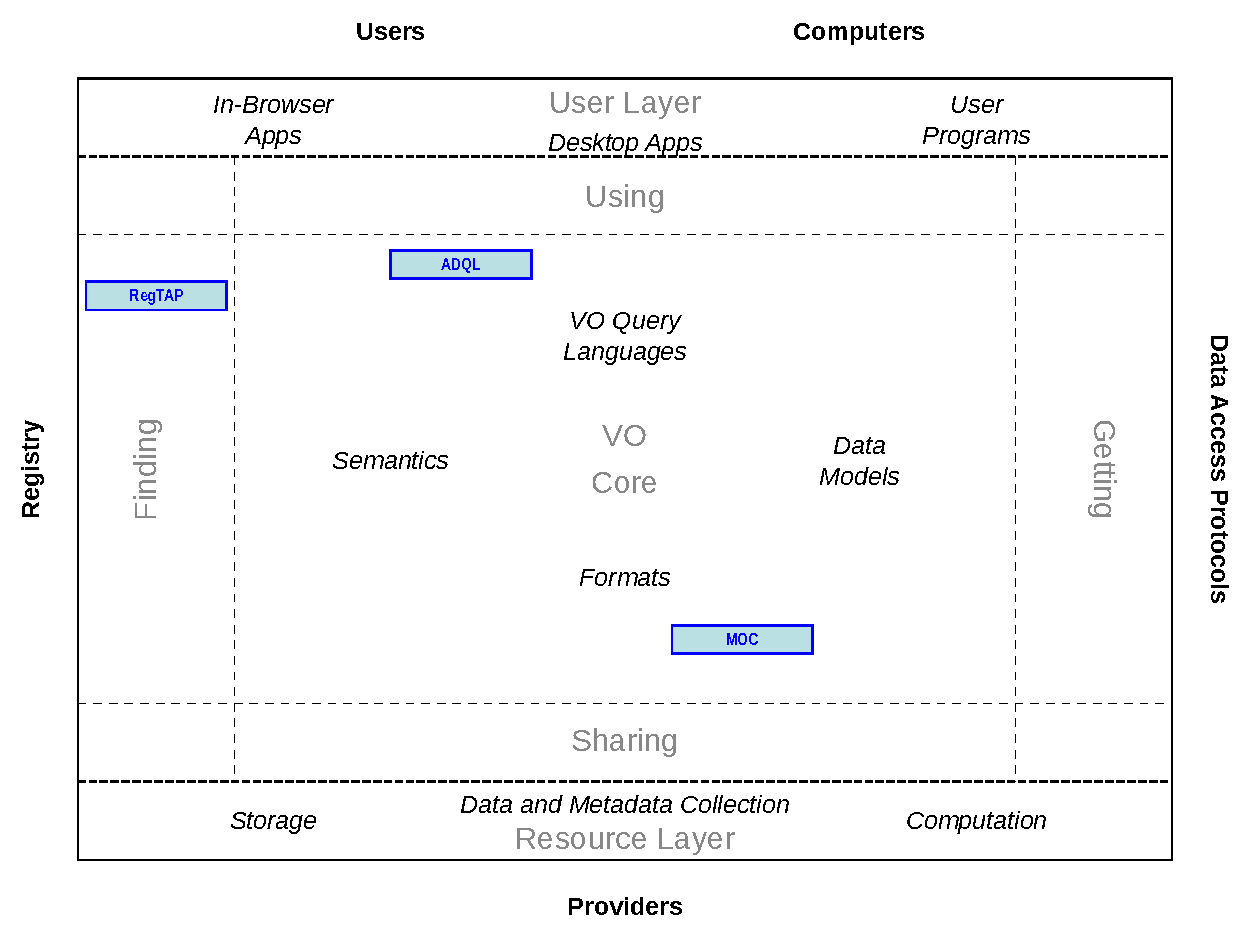
\includegraphics[width=0.9\textwidth]{role_diagram.pdf}
%\caption{Architecture diagram for this document}
%\label{fig:archdiag}
%\end{figure}

%Fig.~\ref{fig:archdiag} shows the role this document plays within the
%IVOA architecture \citep{note:VOARCH}.

%???? and so on, LaTeX as you know and love it. ????

\section{List of IVOA user defined functions}
\subsection{Healpix related}
\subsubsection{\texttt{ivo\_healpix\_index} with ra and dec}

Parameters:

\begin{itemize}
	\item hpxOrder (\texttt{INTEGER})
	\item ra (\texttt{DOUBLE})
	\item dec (\texttt{DOUBLE})
\end{itemize}

Returns: \texttt{BIGINT}

Returns the index of the (nest) Healpix cell at the specified order
hpxOrder containing the specified spherical point defined as a right
ascension and declination value.

\subsubsection{\texttt{ivo\_healpix\_index} with an spherical point}

Parameters:

\begin{itemize}
	\item hpxOrder (\texttt{INTEGER})
	\item point (\texttt{POINT})
\end{itemize}

Returns: \texttt{BIGINT}

Returns the index of the (nest) Healpix cell at the specified order
hpxOrder containing the specified spherical point.

\subsubsection{ivo\_healpix\_center}

Parameters:

\begin{itemize}
	\item hpxOrder (\texttt{INTEGER})
	\item hpxIndex (\texttt{INTEGER})
\end{itemize}

Returns a \texttt{POINT} corresponding to the center of the Healpix cell
with the given index at the given order.

\subsubsection{\texttt{ivo\_apply\_pm}}

Parameters:

\begin{itemize}
	\item ra (\texttt{DOUBLE})
	\item dec (\texttt{DOUBLE})
	\item pmra (\texttt{DOUBLE})
	\item pmdec (\texttt{DOUBLE})
	\item epochDist (\texttt{DOUBLE})
\end{itemize}

Returns: \texttt{POINT}.

Returns a \texttt{POINT} for a given proper motion (prma and pmdec)
after a given number of Julian years. Positions must be in degrees,
proper motions are expected in degrees/year. Pmra is assumed to contain
cos(delta).

\subsection{Text related}

\subsubsection{ivo\_string\_agg}

Parameters:

\begin{itemize}
	\item expression (\texttt{TEXT})
	\item delimiter (\texttt{TEXT})
\end{itemize}

Returns: \texttt{TEXT}

An aggregate function returning all values of expresion within a GROUP
concatenated with delimiter.

\subsubsection{ivo\_nocasematch}

Parameters:

\begin{itemize}
	\item value (\texttt{TEXT})
	\item pattern (\texttt{TEXT})
\end{itemize}

Returns: \texttt{INTEGER}

Pattern is defined as for the SQL LIKE operator, but the match is
performed case-insensitively. This function in effect provides a
surrogate for the ILIKE SQL operator that is missing from ADQL. Returns
1 if pattern matches, 0 otherwise.

\subsubsection{ivo\_hasword}

Parameters:

\begin{itemize}
	\item haystack (\texttt{TEXT})
	\item needle (\texttt{TEXT})
\end{itemize}

Returns: \texttt{INTEGER}.

This is for "google-like" searches in text-like fields. In word you can
employ a fairly complex query language; see
http://postgresql.org/docs/8.3/static/textsearch.html for details.
Returns 1 if needle shows up in haystack, 0 otherwise.

\subsubsection{ivo\_hashlist\_has}

Parameters:

\begin{itemize}
	\item hashlist (\texttt{TEXT})
	\item item (\texttt{TEXT})
\end{itemize}

Returns: \texttt{INTEGER}

Takes two strings, the first is a list of words not containing the hash
sign (\#), concatenated by hash strings; the second is a word not
containing the hash sign. It returns 1 if, compared case-insensitively,
the second argument is in the list of words coded in the first argument.
The behaviour in case the second argument contains a hash sign is
unspecified.

\subsection{Other}

\subsubsection{ivo\_internal\_overlaps}

Parameters:

\begin{itemize}
	\item l1 (\texttt{NUMERIC})
	\item h1 (\texttt{NUMERIC})
	\item l2 (\texttt{NUMERIC})
	\item h2 (\texttt{NUMERIC})
\end{itemize}

Returns \texttt{INTEGER}.

The function returns 1 if the interval [l1...h2] overlaps with the
interval [l2...h2]. For the purposes of this function, the case l1=h2 or
l2=h1 is treated as overlap. The function returns 0 for non-overlapping
intervals.

\subsubsection{ivo\_interval\_has}

Parameters:

\begin{itemize}
	\item val (\texttt{NUMERIC})
	\item iv (\texttt{INTERVAL})
\end{itemize}

Returns \texttt{INTEGER}.

The unction returns 1 if the interval iv contains val, 0 otherwise. The
lower limit is always included in iv, behaviour on the upper limit is
column-specific.

\section{List of third-party user defined functions}

In this section those functions deemed necessary but not
\textit{official} or IVOA-sanctioned will be added. Currently, these
entities are represented:

\begin{enumerate}
	\item GAVO
\end{enumerate}

\subsection{GAVO functions}

\subsubsection{gavo\_simbadpoint}

Parameters:

\begin{itemize}
	\item identifier (\texttt{TEXT})
\end{itemize}

Returns \texttt{POINT}.

Queries Simbad for an identifier and returns the corresponding point.
Note that identifier can only be a literal, i.e., as simple string
rather than a column name. This is because the GAVO database cannot
query Simbad, and probably wouldn't want to fire of millions of Simbad
queries anyway; use Simbads's own TAP service for these kind of
applications.

\subsubsection{gavo\_to\_jd}

Parameters:

\begin{itemize}
	\item d (\texttt{TIMESTAMP})
\end{itemize}

Returns \texttt{DOUBLE PRECISION}.

Converts a postgres timestamp toi a modified julian date. This is naive;
no corrections for timezones, let alone time scales or the like are done;
you can thus not expect this to be good to second-precision unless you
are careful in the construction of the timestamp.

\subsubsection{gavo\_to\_mjd}

Parameters:

\begin{itemize}
	\item d (\texttt{TIMESTAMP})
\end{itemize}

Returns \texttt{DOUBLE PRECISION}.

Converts a postgres timestamp to julian date. This is naive; no
corrections for timezones, let alone time scales or the like are done;
you can thus not expect this to be good to second-precision unless you
are careful in the construction of the timestamp.

\subsubsection{gavo\_histogram}

Parameters:

\begin{itemize}
	\item val (\texttt{REAL})
	\item lower (\texttt{REAL})
	\item upper (\texttt{REAL})
	\item nbins (\texttt{INTEGER})
\end{itemize}

Returns: \texttt{INTEGER\[\]}

The aggregate function returns a histogram of val with nbins+2 elements.
Assuming 0-based arrays, results[0] contains the number of underflows
(i.e., val<lower), result[nbins+1] the number of overflows. Elements
i..nbins are the counts in nbins bins of width (upper-lower)/nbins.
Clients will have to convert back to physical units using some external
communication, there currently is no (meta-) data as lower and upper in
the TAP response.

\subsubsection{gavo\_transform}

Parameters:

\begin{itemize}
	\item from\_sys (\texttt{TEXT})
	\item to\_sys (\texttt{TEXT})
	\item geo (\texttt{GEOMETRY})
\end{itemize}

Returns: \texttt{GEOMETRY}.

Transforms ADQL geometries between various reference systems. GEO can be
a \texttt{POINT}, a \texttt{CIRCLE}, or a \texttt{POLYGON}, and the
function will return a geometry of the same type. In the current
implementation, from\_sys and to\_sys must be literal strings (i.e.,
they cannot be computed though expressions or be taken from database
columns).

\subsubsection{gavo\_ipix}

Parameters:

\begin{itemize}
	\item long (\texttt{REAL})
	\item lat (\texttt{REAL})
\end{itemize}

Returns: \texttt{BIGINT}.

Returns the q3c ipix for a long/lat pair (it simply wraps the
\texttt{13c\_angpix} function). Probably relevant when playing tricks
with indices of PPMXL ids.

\appendix

\section{Methodology to obtain this catalogue}

A small script has been written to obtain the different UDF used
throughout the registry. It is not perfect and should be subject of
review and change.

\section{Changes from Previous Versions}

No previous versions yet.  
% these would be subsections "Changes from v. WD-..."
% Use itemize environments.


\bibliography{ivoatex/ivoabib,ivoatex/docrepo}


\end{document}
